\documentclass{article}
\usepackage{etoolbox}
\usepackage{graphicx}

\ifdef{\myoutput}{}{\def\myoutput{concept}}
\ifdef{\myversion}{}{\def\myversion{1}}

\usepackage[output=\myoutput
,numberofversions=4
,version=\myversion
,seed=4
,randomizequestions=true
,randomizeanswers=true
,writeRfile=true
]{mcexam}

\usepackage[margin=0.95in]{geometry}
\usepackage{multicol}

\usepackage{fancyhdr,lastpage}
\pagestyle{fancy}
\fancyhf{}
\renewcommand{\headrulewidth}{1pt} 
\renewcommand{\footrulewidth}{1pt}
\lfoot{\mctheversion}
\rfoot{Page \thepage\ of \pageref{LastPage}}
\lhead{Quiz 6.3 and 7.1 \mctheversion \\ MAT 2000: Introduction to Statistics}
\rhead{Name Print): \hspace{2.5 in}}

\usepackage{calc}
\renewenvironment{setmcquestion}
{\begin{minipage}[t]{\linewidth-\labelwidth}}
	{\end{minipage}\par}
	
\renewenvironment{setmcquestioninstruction}
{\begin{minipage}{\textwidth}}
	{\end{minipage}}
	
\renewenvironment{setmcanswers}{}{}
\setlist[setmcquestions]{label=\mcquestionlabelfmt{*}.
	,ref=\mcquestionlabelfmt{*}
	,itemsep=0.5\baselineskip
	,topsep=1\baselineskip
}

\renewcommand\mcversionlabelfmt[1]{\arabic{#1}}

%copy-pasting from MS Word, use regex to find [\*]*[a-d]\. and replace with \answer 

\raggedbottom

\begin{document}
	Circle the correct answer for each question.  If you're unsure, you can write numbers 1, 2, 3, etc. next to the choices to get partial credit.\\[.5cm]
	
	\begin{mcquestions}
		\begin{mcquestioninstruction}
			The Women's Health Study included 39,876 female health professionals aged 45 years and older who were followed for an average of 10 years (Ridker et al., 2005). At the beginning of the study, participants were randomly assigned to take either a daily low-dose aspirin or a daily placebo pill for the duration of the study. At the end of the study, researchers measured the number of participants that suffered from a heart attack during the study. Data are summarized in the following table.
			\begin{tabular}{llll}
								& Low-dose Aspirin	& Placebo	& Total\\
				Heart Attack	& 198				&	193		&	391\\
				No Heart Attack	& 19,736			&	19,749	& 39,485\\
				Total			&	19,934			&	19,942	& 39,876
			\end{tabular}
		\end{mcquestioninstruction}
		
		\question Is a theory-based approach appropriate to evaluate the relationship between whether an individual took aspirin or a placebo and whether an individual suffers a heart attack?
		\begin{mcanswerslist}
			\answer No, since a simulation-based approach is always appropriate.
			\answer Yes, since 39,876 is larger than 20.
			\answer[correct] Yes, since 198, 193, 19,736, and 19,749 are all greater than 10.
			\answer Yes, since 391 and 39,485 are both greater than 10.
		\end{mcanswerslist}
		
		\question[follow] Based on a 95\% confidence interval $(-0.0014, 0.0019)$ for the data above, what could be said for sure about the p-value for testing
		$H_0 : \pi_a - \pi_p = 0$ versus $H_A : \pi_a - \pi_p \neq 0$?
		\begin{mcanswerslist}
			\answer p-value < 0.01
			\answer[correct] p-value < 0.05
			\answer p-value < 0.10
			\answer p-value > 0.10
		\end{mcanswerslist}
		
		\question For a confidence interval, if the confidence level from 95\% to 99\%, all else remaining the same, how would the center of the confidence interval be affected?
		\begin{mcanswerslist}
			\answer Increase
			\answer[correct] Remain the same
			\answer Decrease
			\answer Cannot be determined
		\end{mcanswerslist}
		
		\question For a confidence interval, if the confidence level from 95\% to 99\%, all else remaining the same, how would the the width of the confidence interval be affected?
		\begin{mcanswerslist}
			\answer[correct] Increase
			\answer Remain the same
			\answer Decrease
			\answer Cannot be determined
		\end{mcanswerslist}
		
		\begin{mcquestioninstruction}
			Monthly snowfall (in inches) was measured over several winters in Fort Collins, Colorado. Researchers also recorded whether the measurement was taken in the Early winter (September to December) or Late winter (January to June). Boxplots displaying the distribution of monthly snowfall for each season are below.
			\begin{center}
				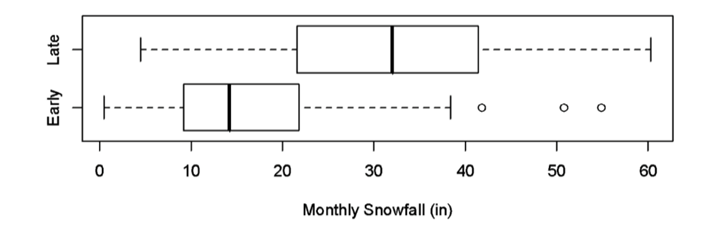
\includegraphics[width=\textwidth]{snowfall.png}
			\end{center}
			Use this to answer the next five questions:
		\end{mcquestioninstruction}
		
		\question The shape of the distribution of monthly snowfall measurements for the Early season is
		\begin{mcanswerslist}
			\answer symmetric.
			\answer[correct] skewed right.
			\answer skewed left.
			\answer bimodal.
		\end{mcanswerslist}
		
		\question[follow] What is the upper quartile (Q3) of the distribution of monthly snowfall measurements for the Late season (approximately)?
		\begin{mcanswerslist}
			\answer 22
			\answer 33
			\answer[correct] 41
			\answer 60
		\end{mcanswerslist}
		
		\question[follow] Which of the following sentences correctly interprets the first quartile (Q1) of the distribution of monthly snowfall measurements for the Early season?
		\begin{mcanswerslist}
			\answer[correct] About 25\% of Early season winter months in Fort Collins get less than 9 inches of snow.
			\answer About 50\% of Early season winter months in Fort Collins get less than 9 inches of snow.
			\answer About 75\% of Early season winter months in Fort Collins get less than 9 inches of snow.
			\answer About 25\% of Early season winter months in Fort Collins get more than 38 inches of snow.
		\end{mcanswerslist}
		
		\question[follow] Which season has the larger median monthly snowfall?
		\begin{mcanswerslist}
			\answer Early
			\answer[correct] Late
			\answer The two medians are approximately equal.
			\answer The plot does not provide enough information to determine which median is larger.
		\end{mcanswerslist}
		
		\question[follow] The boxplots demonstrate that there is an association between which two variables?
		\begin{mcanswerslist}
			\answer Early and Late winter season
			\answer Snowfall and months
			\answer[correct] Monthly snowfall and whether the time was Early or Late winter season
			\answer Whether it was Early or Late winter season and months
		\end{mcanswerslist}
		
		\question Which of the following data sets has the largest standard deviation?
		\begin{mcanswerslist}
			\answer 1, 2, 3, 4, 5
			\answer 1, 3, 3, 3, 5
			\answer[correct] 1, 1, 3, 5, 5
			\answer 1, 1, 1, 1, 1
		\end{mcanswerslist}
		
	\end{mcquestions}
\end{document}